\section{Experimental Evaluation}
\label{sec:experiments}

We evaluate the execution choices of Section~\ref{sec:algorithms} in a
bounded, reproducible pilot. The questions are whether the exact-greedy
implementations agree, how their setup and search costs compare with the
full ILP, and how signed-threshold greedy behaves for AVG. The experiment
uses TPC-H data~\cite{tpch} with a derived scalar query, rather than the
standard TPC-H query suite or its throughput metric.

\subsection{Workload and Measurement Protocol}

The query joins Customer, Orders, Lineitem, and Part on their standard
foreign keys and selects line items shipped in January 1995. Only Customer
and Part tuples are deletable; Orders and Lineitem are immutable. Each
surviving join derivation contributes one COUNT input or its extended price
for SUM and AVG. Prices are represented in integer cents. The two existing
TPC-H databases have scale factors 0.01 and 0.03, yielding respectively
714 and 2,358 derivations, and 949 and 3,128 contributing deletable tuples.
All supports have rank two. We use downward changes of 10\%, 25\%, and
50\% of the initial COUNT/SUM answer, rounding the required loss upward
to an integer. For AVG we use exact rational targets 2\%, 5\%, and 10\%
below its initial value.

The COUNT/SUM methods are: (i) the full survival-variable ILP of
Section~\ref{sec:ilp}; (ii) incremental-support greedy with a scan for the
largest gain; (iii) certified lazy greedy whose marginal queries run in
SQL on a materialized derivation table; and (iv) a circuit pass computing
the exact derivatives of
\[
P(y)=\sum_c y_c\sum_{b:\,c_b=c}w_b y_{p_b}.
\]
This last method specializes the multilinear oracle to the workload's
Customer/Part supports. It evaluates the inner sums and their derivatives
directly; circuit compilation and compression are separate questions.
AVG compares the full ILP with the net signed-gain heuristic of
Section~\ref{sec:avg-search}.

The machine uses an Apple M5, macOS, and Python 3.9.6. Methods run
sequentially with DuckDB 1.4.3~\cite{duckdb2019}, PuLP 3.3.0, and
HiGHS 1.12.0~\cite{highs}.
DuckDB and HiGHS use one thread. Each ILP has a five-second solve limit
and zero requested MIP gaps. Each combination of scale, aggregate, and threshold is repeated
three times, with algorithm order shuffled using seed 1729.
These are timing repetitions on fixed inputs. The 18 cases yield 180
method runs, including 54 ILP runs. Method time includes initialization,
model construction or SQL materialization, and optimization. Shared
source extraction and independent verification are excluded; extraction
took 6.3--6.9\,ms per database. We report medians and min/max timing ranges.

For every returned set, we recompute both the surviving derivation bag and
the residual SQL aggregate on the original database. Integer/rational
checks enforce the threshold and, for AVG, nonemptiness. We also require
identical selection traces for the three exact-greedy implementations.
The records retain each witness, solver status and bound, repetition,
input digest, and environment information. The accompanying experiment
artifacts include an analysis script that audits these records and
regenerates the table and figure.

% Generated by experiments/summarize_review.py from frozen measurements.
\begin{table}[t]
\centering
\caption{Optimal witness sizes in the TPC-H-derived pilot. Every measured greedy variant attained these sizes; each case has three timing repetitions.}
\label{tab:pilot-sizes}
\small
\begin{tabular}{@{}lrrr@{}}
\toprule
Aggregate & Decrease (\%) & SF 0.01 & SF 0.03\\
\midrule
\agg{COUNT} & 10 & 14 & 39\\
\agg{COUNT} & 25 & 40 & 121\\
\agg{COUNT} & 50 & 95 & 311\\
\agg{SUM} & 10 & 11 & 34\\
\agg{SUM} & 25 & 33 & 108\\
\agg{SUM} & 50 & 85 & 276\\
\agg{AVG} & 2 & 7 & 17\\
\agg{AVG} & 5 & 18 & 53\\
\agg{AVG} & 10 & 39 & 121\\
\bottomrule
\end{tabular}
\end{table}


\begin{figure*}[t]
\centering
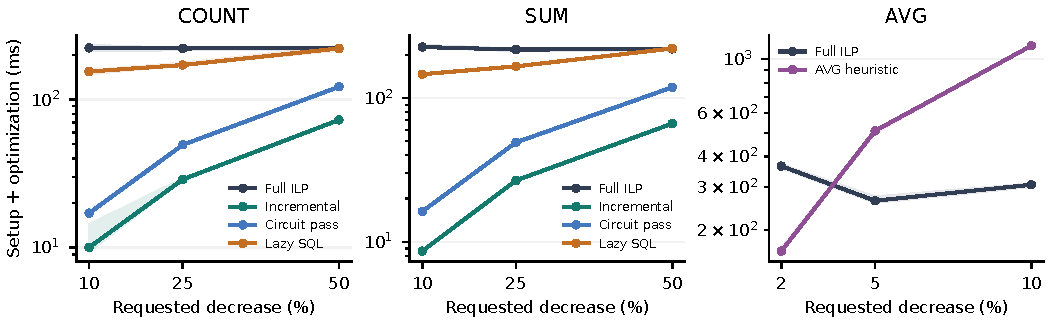
\includegraphics[width=\textwidth]{figures/evaluation_runtime.pdf}
\caption{TPC-H-derived pilot at SF 0.03. Points show median setup-plus-
optimization time over three repetitions; shaded ranges show the observed
minimum and maximum. The SQL method includes derivation-table
materialization. The circuit method is the specialized multilinear pass.
COUNT/SUM and AVG use different decrease ranges.}
\label{fig:pilot-runtime}
\Description{Three line plots compare median setup and optimization times at scale factor 0.03 as the requested decrease grows. Incremental coverage is fastest for COUNT and SUM. The AVG heuristic becomes slower than the full ILP at larger decreases. Shaded bands show the minimum and maximum of three timing repetitions.}
\end{figure*}

\subsection{Results and Interpretation}

\paragraph{Witness quality and correctness.}
All 180 returned sets passed both validation checks, all 54 ILP solves
reported optimality, and no run timed out. The exact-greedy variants agreed
on every selected tuple at each of the 12 COUNT/SUM cases. Their final
sizes matched the proven optimum in every case; AVG greedy also matched
it in all six AVG cases (Table~\ref{tab:pilot-sizes}). This is an observation
about the selected workload. For comparison, a four-derivation COUNT
control with supports $\{a,x\},\{a,y\},\{b,x\},\{c,y\}$ and full-loss
target has optimum $\{x,y\}$, whereas greedy with tuple order
$a,b,c,x,y$ selects $a,b,c$. Thus exact marginal computation does not make
greedy an exact optimization method in general.

\paragraph{Execution costs.}
At SF 0.03 and a 50\% COUNT decrease, median method time is 72.9\,ms for
incremental greedy, 121.9\,ms for the circuit pass, 221.5\,ms for lazy
SQL, and 222.0\,ms for ILP. All return size 311. Incremental greedy is
about $3.0\times$ faster than ILP in this cell. Its gains change only when
incident derivations die, whereas the circuit pass scans the surviving
contributions at every iteration. Lazy SQL reduces repeated gain
computation but also pays for its materialized table and SQL calls.
Figure~\ref{fig:pilot-runtime} shows the measured tradeoff across thresholds.

AVG illustrates a different cost profile. At SF 0.03 and a 10\% average
decrease, both methods return size 121, but the heuristic takes a median
1.132\,s versus 0.307\,s for ILP, about $3.7\times$ longer. The heuristic
repeatedly computes signed rational gains, while these small ILPs solve
quickly. A heuristic label therefore does not imply a runtime advantage.

\paragraph{Evaluation scope.}
The pilot validates three exact coverage implementations and a constructive
AVG search on one self-join-free join shape at two small scales. The timing
ranges characterize repeated execution of these inputs, rather than
variation across datasets. Larger databases, additional join shapes,
self-joins, extrema survivor enumeration, and peak memory remain necessary
dimensions of a broader scalability study. These distinctions keep
representation-level speedups separate from end-to-end workload claims.
